\documentclass{article}
\usepackage{listings}
\usepackage[utf8]{inputenc}
\usepackage{fancyhdr}
\usepackage{xcolor}
\usepackage{caption}
\usepackage{graphicx}
\usepackage{algpseudocode}
%\usepackage{amsmath}
%\usepackage{booktabs}
%\usepackage{textcomp}
%\usepackage{rotating}
\usepackage{libertinus}
\usepackage{libertinust1math}
\usepackage{float}
\usepackage{lipsum}
\usepackage[T1]{fontenc}
\usepackage[english]{babel}

% === Colours ===
\definecolor{codegreen}{rgb}{0,0.6,0}
\definecolor{codegray}{rgb}{0.5,0.5,0.5}
\definecolor{codepurple}{rgb}{0.58,0,0.82}
\definecolor{backcolour}{rgb}{0.95,0.95,0.92}
% === End Colours ===

% === Layout ===
\setlength{\parskip}{0.5em}
\graphicspath{ {./images/} }
\lstdefinestyle{code}{basicstyle=\ttfamily\footnotesize, breakatwhitespace=false,
    breaklines=true, keywordstyle=\color{magenta}, commentstyle=\color{codegreen},
    keepspaces=true, showspaces=false, showstringspaces=false}
\lstset{style=code}
\pagestyle{fancy}
\fancyhf{}

\rhead{Callum Donovan}
\lhead{Implementing SAT Algorithms in Software}
\rfoot{Page \thepage}
\lfoot{CS-M20 - 1915769}
\title{\bfseries Implementing SAT Algorithms in Software}
\author{Callum Donovan}
\date{ \today }
% === End Layout ===

\begin{document}

% === Title Page ===
\begin{titlepage}
    \begin{center}
        \Large{\bfseries Implementing SAT Algorithms in Software} \\
        \vspace*{\fill}
        \begin{center}
            
\includegraphics[scale=0.15]{swan.jpg}
        \end{center}
        \vspace*{\fill}
        \bfseries{\large Callum Donovan \\
            1915769 \\
            \today \\
            Swansea University \\}
    \end{center}
\end{titlepage}
% === End Title Page ===

% === Main Content ===
\thispagestyle{empty}
\begin{center}
\section*{Abstract}
\end{center}
% TODO: Use the word "implement" a lot less!
The Boolean Satisfiability Problem is a fundamental part of Computer Science. First proven to be an
NP-Complete problem by both Stephen Cook in 1971\cite{scook}, and Leonid Levin in 1973\cite{levin}. Since then, many more
NP-Complete problems have been identified, along with their respective uses in the real world
outside of pure computer science. Due to this, there has been a growing need for solvers that can
effectively and efficiently process these problems. In the last two decades alone, huge progress has
been made to coincide with the advancements in technology. And more SAT solvers have appeared that
can be deployed in industries where they are most needed.

This paper explores the basic concept behind SAT solvers, and how they can be implemented in
software using modern programming languages and tools. The algorithm that will be
implemented is one proposed by Donald Knuth in his book "The Art of Computer Programming". Knuth proposes
many algorithms, ranging from the most basic backtracking based algorithm, to an advanced
implementation of WalkSAT[!]. We will explore the fundamentals of how to implement these algorithms,
implement one of them, then test its performance against a suite of SAT problems.

The result of this paper will be a SAT solver implemented in C++, using the data structures and
steps provided by Donald Knuth in his book "The Art of Computer Programming".

\newpage
\thispagestyle{empty}
\tableofcontents

\newpage
\section{Introduction}
% TODO: Refactor to sound better.
% TODO: Add some examples to interest the reader.
Satisfiability has presented itself a huge area of research throughout the history of computer
science. Being the first proved to be NP-Complete in 1971\cite{scook}, it has been the go-to for complex
computation. And using reduction techniques pioneered in the mid-twentieth century, many other types
of complex problems can be converted into SAT and solved using the plethora of solvers freely
available. In more recent years, SAT competitions have added an incentive to the development of more
advanced solvers, such as Minisat, zChaff, and CaDiCaL. On top of these, parallel solvers have
gained popularity and one such solver, called Plingaling, ranked very highly in the SAT Competition
2020. Showing how parallel solvers can be just as good as their counterparts, if not better.

Donald Knuth has taken particular interest in this topic with his recent chapter of "The Art of Computer Programming". He discusses how important SAT solvers are to both industry and research, as well as providing algorithms and sample problems to test them against.

This paper will be an exploration into the world of SAT solvers and how they can provide crucial services to both industry and research. As well as methods in which proposed SAT solver algorithms can be implemented into a robust piece of software. Due to the sheer size of literature and research in this field, it would be unrealistic to think it is possible to cover everything in a comprehensive way. Therefore, this paper focuses on the fundamentals of SAT and the significant research through the years since Cooks paper in 1971\cite{scook}. As well as the ideas presented by Donald Knuth for implementation in modern programming languages.

\subsection{Motivation}

The motivation behind this project stems from the ever growing need for more efficient and faster SAT solvers. But in order to begin researching in this field, one must know the basics and tried methods present today. This project will do just that, in both studying literature that has formed the basis of most of the field, and implementing a basic SAT solver.

One of the most common arguments for the research into SAT solving is its viability for both science and industry. This presents a convenient compatibility between the two. As industry requirements grow, so too does the need for research into better algorithms to satisfy those requirements. An example in which SAT solvers are a key part of industry include Electronic Design Automation (or EDA). We will explore these usages further as we progress and highlight the advantages of fast SAT solvers when applied to these industries.

Another common viability for SAT solvers includes their usage for most complex problems that can be reduced to SAT. Most problems in the real world can be cast as optimisation problems. This allows us to create a mathematical description of these problems, which in turn can present themselves for solving. The use of a solver in this instance would produce results which would allow for cost-saving or general efficiency improvements.

\subsection{Aims and Objectives}
% TODO: Refactor this section, especially the DK bit.
To preface this project we must present the aims and objectives that we wish to aim for. As explained above, we do not wish to push the boundaries of SAT solvers in this particular project. But instead want to explore the basics and expand on current research. Aiding us in this goal will be the series by Donald Knuth, "The Art of Computer Programming". Knuth has recently taken interest in the concept of satisfiability for "Fascicle 6: Satisfiability" , and presents a large amount of content for us to analyse. In this book, Knuth outlines multiple algorithms that could be used to implement multiple common SAT solvers. These include:

\begin{itemize}
    \item Algorithm B - Backtracking with watched literals.
    \item Algorithm D - DPLL.
    \item Algorithm C - CDCL.
    \item Algorithm L - DPLL with lookahead.
    \item Algorithm W - WalkSAT.
\end{itemize}

% Be careful of the spell checker attempting to "americani(z)e" everything.
We shall be analysing one of these algorithms and presenting the data structures needed and methods of implementation using C++. Once our implementation is complete, and testing has proved the solver to be working as intended, we will record the performance metrics in a scientific manner to ensure accuracy. These metrics will then be compared to other FOSS solvers that are well tested and commonly used. This will give us a benchmark as to how increasing complexity of the algorithm and program can achieve greater performance. As well as how the programming language chosen can effect the overall performance.

We can easily turn these actions into functional and non-functional requirements. Doing so will allow us to test against the requirements stated and compare the expected result to the actual result. This format matches a more "software engineering" approach, which is desired for this project.

\subsubsection{FREQ1}
The resulting software should be able to process an input CNF formula in the semi-standard DIMACS format.

\subsubsection{FREQ2}
% TODO: Clarify this, 'short amount of time' doesn't seem very scientific.
The resulting software should be able to evaluate the satisfiability of a simple formula from FREQ1, and return the result when found. Simple refers to a formula which most SAT solvers would be able to process in a short amount of time. Result refers to the decision returned from the solver that concludes as "SATISFIABLE" or "UNSATISFIABLE".

\subsubsection{Non-Functional Requirements}
These requirements differ from functional requirements as they are not crucial to the project's success. These are simply goals that, if time allows, can be implemented for further data.

\subsubsection{NFREQ1}
The resulting software should be able to process a complex formula within a reasonable amount of time. Reasonable refers to the length of time it takes to return a result when compared to other SAT solvers, i.e. 300 seconds to return "SATISFIABLE".

%\begin{itemize}
%    \item To make a SAT solver using instructions from "TAOCP"
%    \item Make sure the solver can solve generic problem sets in DIMACS.
%    \item Make sure the solver can do this in a decent amount of time.
%    \item Basically FREQ1 and FREQ2.
%\end{itemize}

\subsection{Methodology}
This project is not being shared amongst a large team of engineers. This allows us to choose from a plethora of software methodologies that would typically not be considered. The usual norm is to commit to the AGILE methodology no matter the project. But for us we do not need the potentially cumbersome nature that can come from AGILE. We also need to consider the idea of rapid prototyping and development. For this reason, we have chosen to use the traditional Waterfall methodology. It gives us the general structure for the project, and fits well with our rigid requirements.

\section{Background}
Before we get into the implementation and software, it is always good to have a solid understanding
of the topic at hand. SAT in particular is quite a deep topic, it is easy to spend a long time
researching into all the intricacies[!]. For this paper, we will just be concentrating on the
general concepts and ideas behind 3SAT problems.

\begin{itemize}
    \item Maybe include some complex problem sets here?
\end{itemize}

% TODO: Insert previous CSCM10 research here, cause we ain't doing it again!

\subsection{SAT Fundamentals}
% TODO: Explain the fundamentals of SAT and the people who found it.
\begin{itemize}
    \item Define the SAT problem with reference.
    \item Explain how SAT formulas are constructed.
    \item Explain early attempts to solve SAT formulas.
    \item Discuss the DPLL algorithm, the first computer implementation of a solver.
\end{itemize}

\subsection{3SAT}
\begin{itemize}
    \item Define 3SAT.
    \item Show a problem that would be considered 3SAT.
    \item Explain why 3SAT is of particular interest.
\end{itemize}

\subsection{Modern SAT}
\begin{itemize}
    \item Talk about how SAT has evolved since the original DPLL.
    \item Modern SAT competitions.
    \item Parallel SAT solvers.
    \item General future SAT solver stuff.
\end{itemize}

\section{Related Work}
% TODO: Add related work, such as alternative FOSS solutions.
Moving on from the background of SAT, we can look into existing solutions that are freely available.
As of 2020, there are plenty of FOSS programs that can be used to solve large sets of problems. This
is in part due to the regularity of the SAT competitions that encourage people to build
groundbreaking solvers.

\subsection{Minisat}
A popular and early solver that has won many competitions[!] is Minisat. Written in C++ and boasting
just a mere few hundred lines of code, Minisat has been proven to be an effective tool for medium
sized problem sets. First written in 2003 by Niklas Een[!] and Niklas Sorensson[!], its primary goal
was to help developers and researchers get into the field of SAT solving by providing a simple
interface and minimal codebase.

\begin{itemize}
    \item Talk about Minisat.
    \item Go into detail about offshoots from Minisat, such as CryptoMiniSat.
    \item Newer CDCL algorithms.
    \item Look into SAT 2020 to find some interesting new solvers.
    \item Basically talk about applications then the research currently happening.
\end{itemize}

\subsection{CryptoMiniSat}
As the name suggests, this solver builds upon the foundations laid by Minisat to create an all in
one solution to multiple problems. CryptoMiniSat implements most of the useful features from Minisat
2.0 core, along with PrecoSat and Glucose to try to make a one-stop solution. CryptoMiniSat is still
in active development, hosting their code on GitHub for open collaboration.

% TODO: Add more current SAT solvers.

\section{Design}
\begin{itemize}
    \item Summary of what we would want from a design.
    \item Include the algorithm from Donald Knuth (algorithm D).
    \item Discuss the data structures that we will need to implement based off of DK's ideas.
\end{itemize}

\subsection{Algorithm}
The key to all the most successful SAT solvers are the algorithms. The first SAT solver to be implemented for a computer used the DPLL algorithm. As we previously established, the DPLL algorithm is considered one of the firsts and produced good results for the time. As of 2020, there have been a plethora of improvements to the original DPLL algorithm that has allowed it to keep up with the increasing complexity of problems available. The general pseudocode for the original DPLL algorithm can be written as such:

\begin{figure}[h]
% TODO: Put the DPLL algorithm pseudocode here
% Fix the notations not showing up!
\begin{lstlisting}[language=C++]
    Algorithm DPLL
        Input: A set of clauses C
        Output: A truth value

    Function DPLL(C)
        if C is a consistent set of literals then
            return true;
        if C contains an empty clause then
            return false;
        for every unit clause {L} in C do
            C ← unit-propagate(L, C);
        for every literal L that occurs pure in C do
            C ← pure-literal-assign(L, C);
        L ← choose-literal(C);
        return DPLL(C AND {L}) or DPLL(C AND {not(L)});
\end{lstlisting}
\end{figure}

For our project, the algorithm that we will be interested in is a general DPLL algorithm. As
previously discussed, this is just one of a few algorithms given from Donald Knuth. Although it is
relatively simple, it is a good way to explore the basic idea of software SAT solvers. Forming a
foundation for possible further improvements, much like those explained in algorithm L. Donald Knuth
describes the algorithm in a series of steps, also outlining the data structures that we need to
implement it as he has described.


\begin{itemize}
    \item Discuss algorithms presented by DK.
    \item Discuss which algorithm we are planning to implement.
    \item Talk about the ones we aren't going to anyway?
\end{itemize}
% TODO: Talk about how we've design the code based off of the algorithm and preceding content in the book.

\section{Implementation}
\begin{itemize}
    \item Discuss the general idea of the program, including inputs (DIMACS) and outputs (SAT / NON-SAT).
    \item Discuss the process in which we are going to be solving these problems.
    \item Talk about our tool-chain and related crap.
    \item Talk about the attempts at implementing it.
    \item Show the final implementation.
\end{itemize}

The following will be an in-depth look at the steps we need to consider when implementing our
project. Following the design, this section details the general input and output of the program. As
well as the processing that forms the core of the solver. We will also outline the data structures
that are to be implemented and how they will be integrated with the algorithm to culminate in a
working SAT solver. 

We will also be glazing over the tool-chain and related items that are to be used to create the
solver. This includes the language and the compiler that will be used. As well as the editor and
reasoning behind these choices. 

% These are the basic steps of a computer program.
% Explain to the reader what is included for SAT.
\subsection{Input}
The input of the program will be a CNF formula presented in the DIMACS file format. This file format
is the standard for the SAT competitions and allows for simple parsing of the problem. The format
consists of few elements to ensure the problem is presented cleanly, the first of which being
comments. Comments can be marked using the character \texttt{'c'} followed by a single whitespace
character: 

\begin{center}
    \texttt{c This is a comment line}
\end{center}

Lines prefixed with this will be treated as a
comment and thus will not be parsed as part of the problem. After the comments is a line telling the
SAT solver about the problem it is about to ingest, denoted using the character \texttt{'p'}
followed by a single whitespace character.

\begin{center}
    \texttt{p cnf 255 829}
\end{center}

This line will include the type of problem, followed by the number of clauses then
variables. Following the problem description line is the actual formula. This is presented by either
a positive or negative integer, terminated with a \texttt{'0'}. 

\begin{center}
    \texttt{15 16 17 18 19 20 21 0}
\end{center}

Each line corresponds to a clause formatted in the defined problem type. And each integer represents
a unique variable. Using this format we can create consistent problem files which our solver will be
able to ingest and process easily. An example of a problem formatted in this format is presented
below:

% TODO: Get this to actually center
\begin{center}
    \begin{lstlisting}
        c pigeonhole 2 1
        c label:unsatisfiable
        c label:easy
        p cnf 2 3
        1 0
        2 0
        -1 -2 0
    \end{lstlisting}
\end{center}

This input will be read line by line by the solvers parser, recording the key information that it
needs. After successful parsing we can move on to the processing of this problem.

\subsection{Processing}
%\begin{itemize}
%    \item Discuss how the processing works.
%    \item This is the real meat that basically explains the algorithm.
%    \item I feel it would be best to at least discuss the DPLL algorithm.
%    \item Use content from TAOCP and online.
%\end{itemize}
The processing section of the program pipeline is the most important here. This is where our
algorithm will iterate through each variable and set them to either true or false. The way in which
our program will go about this depends on the algorithm that we have chosen. In this instance we
will explain how the DPLL algorithm presented by Donald Knuth will do this. 

% TODO: Explain how the algorithm processes our input.

\subsection{Output}
% https://web.archive.org/web/20190913185210/http://www.satcompetition.org:80/2004/format-solvers2004.html
%\begin{itemize}
%    \item The output will be "SATISFIABLE" or "UNSATISFIABLE".
%    \item Could also output the best solution.
%    \item Explain the output standard for SAT competitions.
%    \item SAT Competition 2002 output rules (see above comment).
%\end{itemize}

The output of our program is just as important as the input. After all, we want to know how the
solver has gotten to the solution it has ended at. Much like the input, we will be following a
semi-standard format that is outlined at each SAT competition. Using this format will allow us to be
consistent with how most SAT solvers output their solutions. 

The format of the output is somewhat similar to the DIMACS format. In that each line is prefixed
with a single character denoting its purpose, followed by a single whitespace character. The main
difference here being that there is no particular order in which the lines must appear. There are
three distinct types of lines in this format: 

\begin{itemize}
    \item \texttt{'c '}: Denotes a comment line in which the program can output any auxilliary
    information.
    \item \texttt{'s '}: Denotes the line where the solution is presented. This must be either
    'satisfiable', 'unsatisfiable', or 'unknown'. Only one instance of this line is allowed.
    \item \texttt{'v '}: Denotes the values of the solution if one is found.
\end{itemize}

The resulting output should combine all three of these types to create a comprehensive result to the
user. This includes the model that the solver has settled on if the solution is satisfiable. This
will allow for the checking of the answer to ensure its correctness. 

% TODO: Add an example of the output here.

% This is going to be pretty important, attempt to simplify for the reader.
\subsection{Data Structures}
\begin{itemize}
    \item Discuss why we're going to have to implement specific data types.
    \item Provide examples on the types of structures to be used.
\end{itemize}

\subsection{Tool-chain}
The following is a quick overview of the tool-chain that will be used for this project. As these aren't the meat of what the project is about, we shall only spend a short time glazing over the available solutions and those we picked.

\subsubsection{Compiler \& Libraries}
There are multiple compilers available for C++ dependant on the platform. Generally for each of the three most common platforms (Windows, Linux, and MacOS) there are reliable and well tested compiler suites available. The GNU Compiler Collection, or GCC, is considered one of the standard compiler suites for C and C++. GCC has implementations for each of the aforementioned platforms via ports. The Windows implementation in particular is included in a few software development environments that are freely available; MinGW, MSYS2, and Cygwin.

As for Linux, the GCC suite can be installed natively typically using the preferred distro's package manager. For this project the code will be compiled on a Debian based system using the GCC suite. Linux provides a simpler method of developing using C / C++ and streamlines the time from development to testing. Alongside this, the included GDB debugger allows for a simple and lightweight debugging solution. We will also be making use of bash scripts to invoke the software and provide flags to control options, something that can be a little more challenging on a Windows machine.

No development will be carried out on a Macintosh as we simply do not have access to one. Typically these types of software are compiled and run using a Linux system, and thus it would make the most sense to follow the given norm.

\subsubsection{Editor \& Environment}
There are a huge swathe of IDE's and editors available for use and as for which one to use, there isn't a definitive answer. We thought that it would be best to just stick with what we know best, and for this instance that would be Visual Studio Code. Although other IDE's are available that can take a lot of the work out of managing a project. It is not really necessary to use one here. This project will not contain a huge amount of code or files, and general debugging and profiling does not need to be done using bloated IDE's. Visual Studio Code contains a massive inventory of extensions available to give an experience just as rich as an IDE, but without the cumbersome nature of one. As for this project we only need a single extension to get the required development environment:

\begin{itemize}
    \item C / C++
\end{itemize}

It is also important to mention any other environment software aside from the previously mentioned. We are going to be using the \texttt{'time'} command to accurately measure the time metrics of the software from start to completion. This command is available through bash and is invoked at the same time as the program itself. An example of the method in which it can be invoked is as follows:

% TODO: Put the time command here to demonstrate invocation.
\begin{center}
    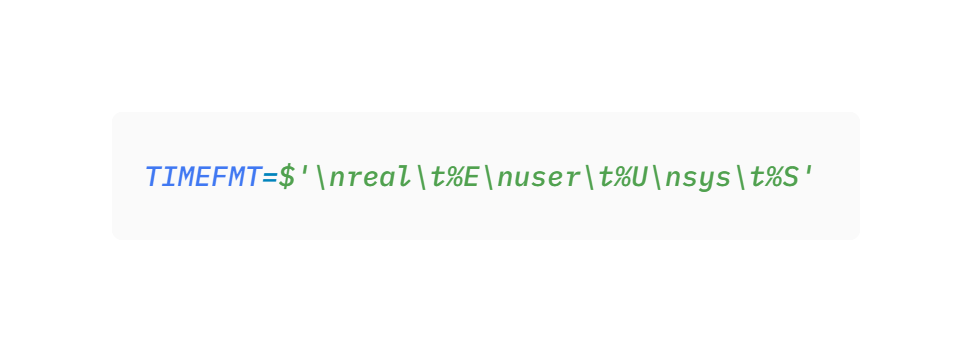
\includegraphics[scale=0.2]{time_command_format.png}
\end{center}

We need to run this command first in order to achieve the desired format. This is only necessary as we are using the
Z-Shell, but the command itself still works the same as traditional Bash. Using the time command we can effectively measure the time that it takes from invocation to completion in a consistent format. This is a simple alternative to implementing a time measuring system into the SAT solver, which could potentially make it less performant. An example of the usage of the time command is shown below:

\begin{center}
    \texttt{\$ time make bin/dpll}
\end{center}

This command will invoke the 'make' binary to compile our program, called dpll. The output of this command will include both the output of the make command, as well as the time it took formatted to our previous rules:

% TODO: Improve the way this looks.
\begin{center}
    \texttt{
        real:   4.70s \\
        user:   2.42s \\
        sys:    0.45s
    }
\end{center}
% TODO: Make this picture look a bit better
%\begin{center}
%    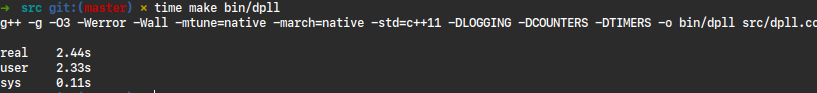
\includegraphics[scale=0.4]{time_command_example.png}
%\end{center}

\subsection{Pseudocode \& Code}
\begin{itemize}
    \item Investigate general pseudocode of generic DPLL algorithm (Wiki).
    \item Create some pseudocode from algorithm.
    \item Create some actual code to show?
\end{itemize}
% TODO: Talk about how we are going to implement this. Not so much about the actual implementation itself!

\section{Testing}
%\begin{itemize}
%    \item Summarize what we want from the testing phase.
%    \item Discuss the problem sets that we are going to be throwing at this.
%    \item Discuss program testing first, even though this is not really what we mean by "testing".
%    \item Record some testing metrics, such as time to solve, memory, CPU cycles, etc.
%    \item Describe any regions that could potentially be improved.
%\end{itemize}
As with all software, one of the most important parts of the development lifecycle is testing. For
this project we must ensure that it not only works without fault, but also returns the correct
results that we are looking for. In order to test our software we shall generate a plethora of
testing criteria to test against. Each of these criteria will have an expected outcome. We will then
compare the expected outcome to the actual outcome and record whether they are identical. Although
this is a simple technique, it is hard to apply automated testing to our program as it is so niche.

As for ensuring the program returns correct results, the best way that we will be able to check is
to use well known and reputable solvers to generate results and compare the two. This can also be
added to the testing criteria and formatted in a table if preferred. The following will be the
details of the testing strategy alongside the results.

\subsection{Software Testing}
%\begin{itemize}
%    \item Discuss methods of software testing (Unit, manual, etc...)
%    \item Outline a testing table for manual testing.
%    \item Discuss testing against the functional requirements stated previously.
%\end{itemize}
There are a vast array of testing tools freely available to use for most software projects. These
have been created from the need for automated testing due to programs changing rapidly. In this
case, we do not need to deploy any advanced testing techniques or tools. As we have quite rigid
requirements and a small codebase, keeping track of changes is somewhat trivial. Much like discussed
in the initial sections of this paper, this is similar to the reasoning behind our choice of
methodology. Therefore, let us create a simple suite of manual testing criteria.

% TODO: Put a testing table here or something.


\subsection{Checking For Correct Solutions}
%\begin{itemize}
%    \item Add results from test folder
%    \item Use two other solvers and give them the same problem
%    \item Check at least 10 times to ensure consistent results
%\end{itemize}
Progressing from the program testing, we must also ensure the solver is returning correct results.
This can also lead us to any bugs that may be present within the program. Using common SAT problems
presented in the DIMACS format we can compare the results from our program to results from another
solver. For statistical reasons we should ensure that each problem set is ran at least 10 times on
each solver. To further back up the testing results we could run the same problems against a third
solver. This would allow for comparison between each solver as a fall-back. 

The first solver we will be using to ensure correctness is \textit{Minisat}. This solver is one of
the most tried and tested solvers freely available to use. And comes with plenty of features to
allow each test set to be completed quickly. \textit{Minisat} comes with a well documented interface
that we can use to easily build and run our test sets. 

% TODO: Run our test set against Minisat.

The fall-back solver we will be using is \textit{CryptoMiniSat}. This solver is still in active
development and encorporates some of the most advanced features for a FOSS solver. Compared to
\textit{Minisat}, this solver is significantly more complex. It should give us safe results that we
can use to ensure no descrepencies between our solver and \textit{Minisat}.

% TODO: Run our test set against CryptoMiniSat.

\subsection{Monitoring Initial Performance Metrics}
%\begin{itemize}
%    \item Measure the performance of this SAT solver (algorithm we picked?)
%    \item Measure the performance of other SAT solvers.
%    \item Compare the results and deduce why the performance differences exist.
%    \item Explain the use of the \texttt{'time'} command with special format.
%\end{itemize}

\subsubsection{UNIX Time Command}
There are multiple ways in which we could measure the performance of the solver. One easy way is measuring the CPU time that the solver takes to give a solution to the problem it is given. This is the reason we will be testing using the standard UNIX 'time' command. This command outputs three metrics; real, user, and system. Real corresponds to the 'wall clock' time that the program took. This refers to the actual time it took from invocation to completion whilst the CPU handles other processes. The 'user' time corresponds to the time the CPU spent on the program in User mode. Calls made in Kernel mode will not be reflected in this time. The 'sys' time corresponds to the time the CPU spent in Kernel mode when executing the program.

These three metrics give us a good idea as to what the CPU spends the most time on when executing our program. This combined with other methods of measuring metrics allow us to assess the performance of the solver more accurately.

\section{Results \& Findings}
\begin{itemize}
    \item Discuss what we found from our testing
\end{itemize}

\section{Evaluation}
\begin{itemize}
    \item Discuss our findings statistically.
    \item Discuss how implemented code could be improved (summarise).
    \item Talk about the methodology we used.
    \item Talk about the risks encountered, and the time frame in which we carried this out.
    \item Discuss the things that could potentially be improved if we did the project again.
    \item Discuss the pandemic.
\end{itemize}

\subsection{Improving Performance}
\begin{itemize}
    \item Explore performance implications of algorithm.
    \item Talk about DK's performance predictions from TAOCP.
    \item Talk about how we could potentially improve the performance of our solver.
    \item Maybe talk about things like parallelism?
\end{itemize}

% TODO: Talk about the challenges we faced and also what we could improve if doing the project again
One of the major issues encountered was something completely out of our control. The Coronavirus pandemic of 2020 provided a massive slew of issues for all academia. Specifically for this project it meant the general plan for the project, as well as the time plan, were both interrupted. The general lockdown for the United Kingdom resulted in confinement to the home. The availability of face-to-face meetings proved to be unfavourable, and potential disruptions in the home delayed planned work.

\section{Conclusion}
\begin{itemize}
    \item Just make a short summary of every single thing that was typed out above!
    \item Don't forget to basically copy and paste this to the abstract.
\end{itemize}
% TODO: Conclude on our findings and all the preceding work we have done.
% === End Main Content ===

% === References ===
\newpage
\bibliographystyle{ieeetr}
\bibliography{references}
% === End References ===

\end{document}
